
\chapter{The EMC effect in SIDIS}
\label{chap:physics}

At this point, it became clear that in order to advance our understanding of the EMC effect, it is necessary to study new observables such as the nucleon virtuality which can be accessible in semi inclusive measurements. Interests for slow nucleons and fragments tagging ($e+A \rightarrow e' + N + X$) studies are older than the EMC effect itself and has been identified earlier to be a promising tool to study nuclear effects~\cite{Frankfurt:1981mk,frankfurt1988,CiofidegliAtti:1993ep}. In more recent work, Melnitchouk {\it et al.}~\cite{Melnitchouk1997} showed that the tagged structure functions of deuteron in $(e,e'N_s)$ semi-inclusive reactions, where $N_s$ denotes the spectator nucleon, is a sensitive probe of the modification of the intrinsic structure of the bound nucleon allowing to discriminate between different EMC models. The extended case to heavier nuclei $A$, where the recoil nucleus $(A-1)$ is tagged was developed by Ciofi degli Atti {\it et al.}~\cite{CiofidegliAtti1999,CiofidelgiAtti:2007qu,Palli2009,Atti:2010yf}, demonstrating the importance of such measurements in the understanding the EMC-type effects. In this proposal, we would like to test experimentally the validity of the spectator mechanism in addition to the investigation of several nuclear effects including final state interactions, medium induced modification of the nucleon structure function and their dependencies on the nucleon binding energy.

\section{The spectator mechanism}


In the spectator mechanism or plane wave impulse approximation, the DIS process corresponds to the absorption of the virtual photon by a quark inside a nucleon, followed by the recoil of the spectator nucleus $A-1$ with low recoil momentum ($\vec P_{A-1}$) and low excitation energy (Fig.~\ref{fig:spectator}). The differential semi-inclusive cross section can be written as~\cite{CiofidegliAtti1999}
\begin{equation}
\sigma_1^A (x_B,Q^2,\vec P_{A-1},y_A,z_1^A)= \frac{d^4\sigma}{dxdQ^2d\vec P_{A-1}} = K^A(x,y_A,Q^2,z_1^A)n_D(|\vec P_{A-1}|)z_1^AF_2^{N/A}(x_A,Q^2,p_1^2),
\label{eq:xs}
\end{equation}
where $Q^2 = -q^2 = -(k_e - k_e')^2 = \vec{q}^{\:2} - \nu$ is the four-momentum transfer, with $\vec{q} = \vec{k_e} - \vec{k_e'}$ and $\nu = E_e - E_e'$, $x_B = Q^2/2 M \nu$ is the Bjorken scaling variable, $p_1 \equiv (p_{10}, \vec{p_1})$, with $\vec{p_1} \equiv - \vec P_{A-1}$, is the four-momentum of the nucleon before its interaction with the virtual photon. $F_2^{N/A}$ is the DIS structure function of the nucleon $N$ in the nucleus $A$, $n_D(|\vec P_{A-1}|)$ is the three-momentum distribution of the bound nucleon, $z^{A}_{1} = {(p_1\cdot q)}/{M\nu}$ is the light cone momentum fraction of the struck quark and $K^A$ is a kinematical factor given by 
\begin{equation}
K^A(x_B,y_A,Q^2,z_1^A) = { 4 \pi \alpha^2 \over Q^4 x_B } \cdot \left( {y \over y_A} \right) ^2 \times \left( {y_A^2 \over 2} + (1-y_A) - {p_1^2x_B^2y_A^2 \over (z_1^A)^2 Q^2 } \right),
\label{eq:ka}
\end{equation}
with $y= \nu / E_e$, $y_A = (p_1 \cdot q)/ (p_1 \cdot k_e)$ and $x_A = x_B / z_1^A$.

Nuclear effects in Eq. \ref{eq:ka} are generated by the nucleon momentum distribution $n_D(|\vec P_{A-1}|)$ and by the quantities $y_A$ and $z^{A}_{1}$, which differ from the corresponding quantities for a free 
nucleon ($y= \nu / E_e$ and $z^{N}_{1} = 1$), if the off-mass shellness of the nucleon ($p_1^2 \neq M^2$) generated by nuclear binding is taken into account.

\begin{figure}[t]
  \begin{center}
    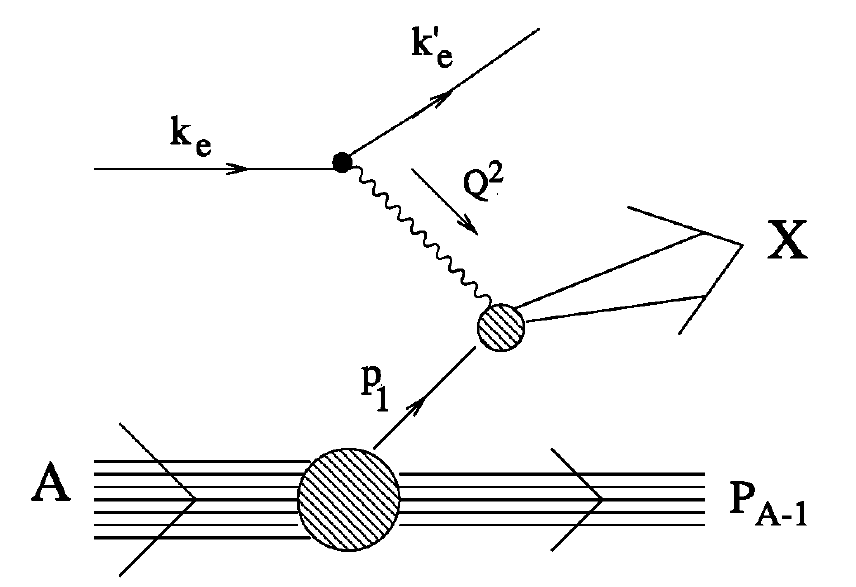
\includegraphics[angle=0, width=0.5\textwidth]{./fig-chap1/spectator}
    \caption{The process $A(e,e'(A-1))X$ within the impulse approximation~\cite{CiofidegliAtti1999}.}
    \label{fig:spectator}
  \end{center}
\end{figure}

To test the spectator mechanism, we use the $\vec P_{A-1}$ dependence of semi-inclusive cross section ratio of different nuclei at the same values of $x_B$, $Q^2$ and $|\vec P_{A-1}| = |\vec P_{A'-1}|$
\begin{equation}
R(x_B,Q^2,|\vec P_{A-1}|,z_1^A,z_1^{A'},y_A,y_{A'})\equiv \frac{\sigma_1^A(x_B,Q^2,|\vec P_{A-1}|,z_1^A,y_A)}{\sigma_1^{A'}(x_B,Q^2,|\vec P_{A'-1}|,z_1^{A'},y_{A'})}.
\label{eq:ratio}
\end{equation}
In the Bjorken limit, the $A$ dependence of $R$ is expected to be entirely dominated by the $A$ dependence of the nucleon momentum distribution $n_D(|\vec P_{A-1}|)$, which exhibits a strong $A$ dependence at low recoil momentum region. Therefore, measurements of the $R$ ratio as a function of the recoil momentum $|\vec P_{A-1}|$ provides a stringent test for the spectator mechanism independently of the model for $F_2^{N/A}$. Fig.~\ref{fig:ratio_spec} illustrates the expected behavior of the ratio in Eq.~\ref{eq:ratio} from the processes D$(e, e' p)X$, $^3$H$(e, e' \mathrm{D})X$ and $^4$He$(e, e'^3 \mathrm{He})X$, as deep inelastic scattering from a bound neutron in different nuclei.

\begin{figure}
  \begin{center}
    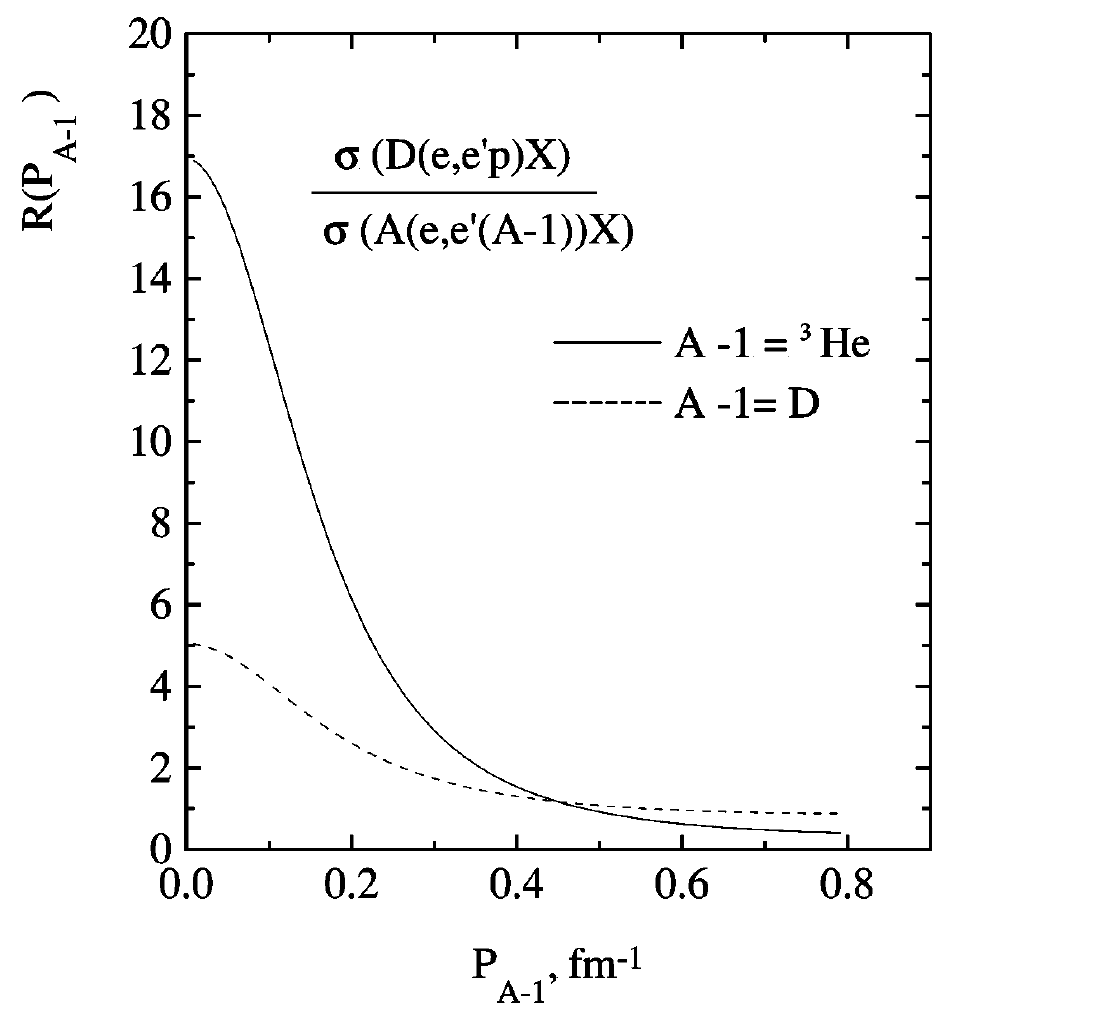
\includegraphics[angle=0, width=0.6\textwidth]{./fig-chap1/ratio_spec}
    \caption{The ratio $R(A,A',|\vec P_{A-1}|)$ for the targets $^3$H (dashed) and $^4$He (full) as a function of the momentum of the backward emitted nucleus~\cite{CiofidegliAtti1999} relative to the virtual photon direction.}
    \label{fig:ratio_spec}
  \end{center}
\end{figure}

From the previous discussion, it is clear that the observation of recoiling nuclei in the ground state, with a $|\vec P_{A-1}|$-dependence similar to the one predicted by the momentum distributions, would represent a stringent check of the spectator mechanism, which, in turns, would indicate the absence of significant Final State Interaction (FSI) between the electro-produced hadronic states and the nuclear medium. Detailed studies~\cite{Melnitchouk1997,CiofidegliAtti2003,ciofi2004,klimenko2006,Alvioli:2006jd,Palli2009} have shown that the FSI effects are minimized in the backward recoiling angle relative to the virtual photon direction and maximized in perpendicular kinematics. The detection of the ground or low energy excited states of the ($A-1$) recoil would represent a strong indication that the hadronization length is larger than the effective nuclear dimension, since if the struck quark hadronizes inside the nucleus, it will likely result in its breakup. The study of~\cite{Palli2009} also pointed out that, for the tagging of slow protons, effects due to the target fragmentation need to be considered. Yet, this mechanism is expected to be pronounced only in the forward direction and for particles with momentum higher than 200 MeV/c. 

\section{EMC effect in deuterium}

\begin{figure}
  \begin{center}
    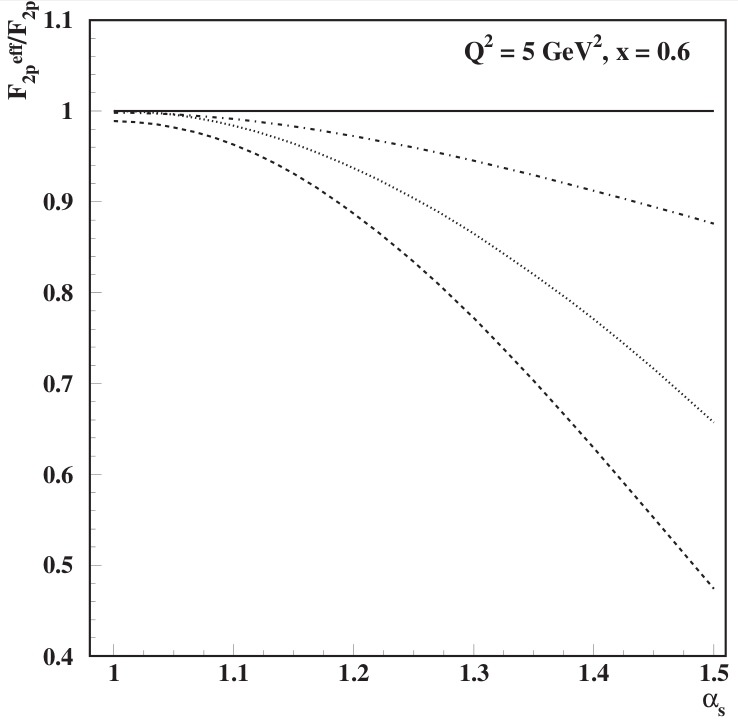
\includegraphics[angle=0, width=0.5\textwidth]{./fig-chap1/plotMel2}
    \caption{$F_{2p}^{eff}$ as a function of $\alpha_s$ for $x = 0.6$ and $p_T = 0$. Dashed line is a prediction for the PLC suppression model, dotted is for the rescaling model, and dot-dashed for the binding/off-shell model \cite{Melnitchouk1997}.}
    \label{fig:mel}
  \end{center}
\end{figure}

The recent finding of the possible dependence of the EMC effect on the local density increased the interest in using spectator nucleons to study the EMC effect. Indeed, the momentum of the spectator nucleon is directly linked to the distance between the two nucleons of deuterium. Beyond the example presented here, other observables can be accessed to probe similar effects and describe in more details the nuclear effect induced by the selection of higher momentum spectators \cite{frankfurt1988,CiofidegliAtti1999,Melnitchouk1997}.

Melnitchouk {\it et al.} \cite{Melnitchouk1997} use the ratio of the effective $F^{eff}_{2p}$ measured in the deuterium, tagging the neutron, and compare it to the usual free $F_{2p}$. They predict significant effects for various models as a function of $\alpha \equiv \displaystyle{{E_s - p_z^s \over M}}$ (with $E_s$ and  $p_z^s$ the energy and longitudinal momentum of the spectator, respectively, and $M$ its mass), which characterizes the nucleon virtuality.  A semi-inclusive measurement will allow to discriminate between the very different model predictions (Fig. \ref{fig:mel}).

We note here the possibility to discriminate between the $x_B$ and $Q^2$-rescaling models, but also more elaborate models, such as the Point Like Configurations (PLC) suppression model. This model, based on color screening, indicates that point like configurations (PLC) \cite{Frankfurt:1985cv,Melnitchouk1997} are rare component of the nucleon wave function, and they might play an important role at $x_B \gtrsim 0.6$. The suppression of the probability to find this configuration in the bound nucleon was offered as yet another explanation of the EMC effect. This model had some success in predicting the $A$ dependence of the EMC effect. The semi-inclusive measurements on deuterium would be used to test further this model as well.

%\begin{figure}
%  \begin{center}
%    \includegraphics[angle=0, width=0.5\textwidth]{./ps_EMC/NNPotential}
%    \caption{Three examples of N-N potential (Bonn~\cite{Machleidt:2000ge}, Reid93~\cite{Stoks:1994wp} and Argonne~V$_{18}$~\cite{Wiringa1995}).}
%    \label{fig:NNpot}
%  \end{center}
%\end{figure}

\section{EMC effect in helium}

The process described for deuterium can be easily extended to heavier nuclei with several advantages. First, the nuclear effects in light nuclei, such as $^4$He, are much stronger, thus it enhances significantly the cross section for events with spectator momentum $\gtrsim 250$~MeV. Second, by detecting an intact light nucleus ($^3$H or $^3$He), we ensure that the final state interaction with the spectator is small and the contributions from the current or target fragmentation of the hard process are suppressed. On the down side, the theoretical calculations are more difficult, however recent theoretical progress indicates that these calculations although tedious could be performed \cite{CiofidegliAtti:1993ep,CiofidegliAtti2003,Alvioli:2006jd,Palli2009}. 

The quantity $R^A$ which is defined by:
\begin{equation}
R^A(x_B,x'_B,Q^2,|\vec P_{A-1}|) \equiv \frac{\sigma_1^A(x_B,Q^2,|\vec P_{A-1}|,z_1^{(A)},y_A)}{\sigma_1^A(x'_B,Q^2,|\vec P_{A-1}|,z_1^{(A)},y_A)},
\label{eq:ratio_a}
\end{equation}
represents the ratio between the cross sections on the nucleus $A$ at two different values of the Bjorken scaling variable. Due to the cancellation of all the other terms but the nucleon structure functions in Eq.~\ref{eq:ratio_a}, $R^A$ is highly sensitive to the nuclear effect. In the binding model ($x$-rescaling), where the inclusive nuclear structure function is expressed through a convolution of the nuclear spectral function and the structure function of the bound nucleon, one has
\begin{equation}
R^A(x_B,x'_B,Q^2,|\vec P_{A-1}|) = \frac{x'_B}{x_B}\frac{F_2^{N/A}(\frac{x_B}{z_1^A},Q^2)}{F_2^{N/A}(\frac{x'_B}{z_1^A},Q^2)}.
\label{eq:x_spec}
\end{equation}
In the $Q^2$-rescaling model~\cite{Close1988}, which is based on the medium modification of the $Q^2$-evolution equations of QCD and the assumption that the quark confinement radius for a bound nucleon is larger than for a free one, the ratio becomes
\begin{equation}
R^A(x_B,x'_B,Q^2,|\vec P_{A-1}|) = \frac{x'_B}{x_B}\frac{F_2^{N/A}(x_B,\xi_A(Q^2)Q^2)}{F_2^{N/A}(x'_B,\xi_A(Q^2)Q^2)}
\label{eq:Q_spec}
\end{equation}

While Eq.~\ref{eq:x_spec} is expected to depend both on $A$ and $|\vec P_{A-1}|$, Eq.~\ref{eq:Q_spec} would be a constant. By detecting nuclei with different recoil angles, this ratio would exhibit different behaviors, allowing a more detailed examination of the dynamics. Fig.~\ref{fig:ratio_a} shows theoretical predictions of the $R^A$ ratio in the $x$- and $Q^2$-rescaling models at both perpendicular and backward recoil kinematics.

\begin{figure}
  \begin{center}
    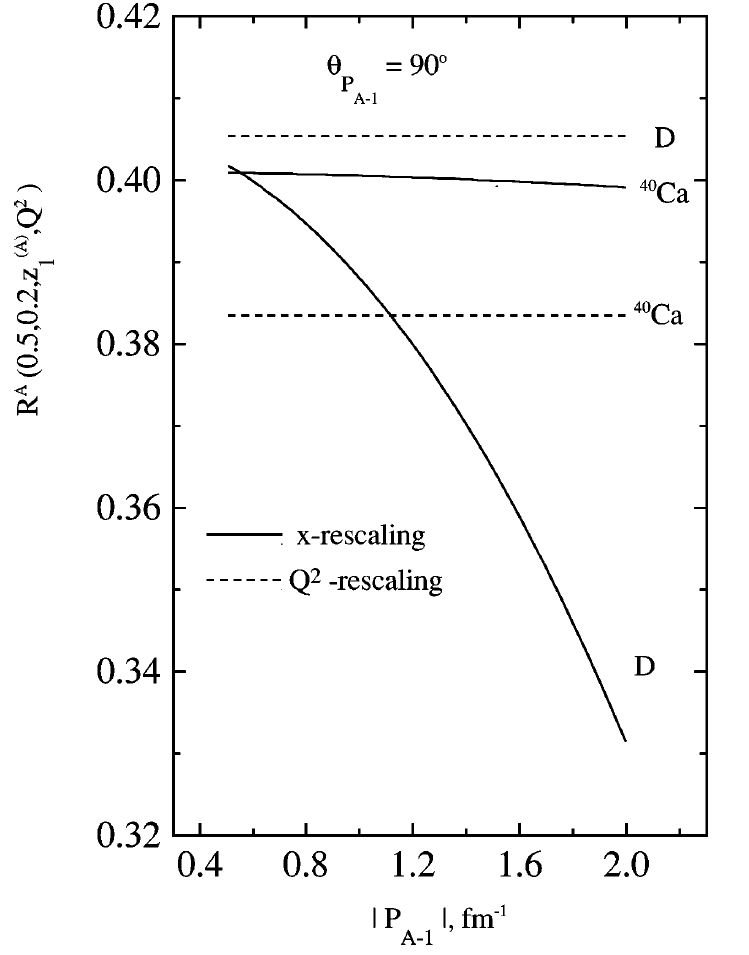
\includegraphics[angle=0, width=0.4\textwidth]{./fig-chap1/ratio_a1}
    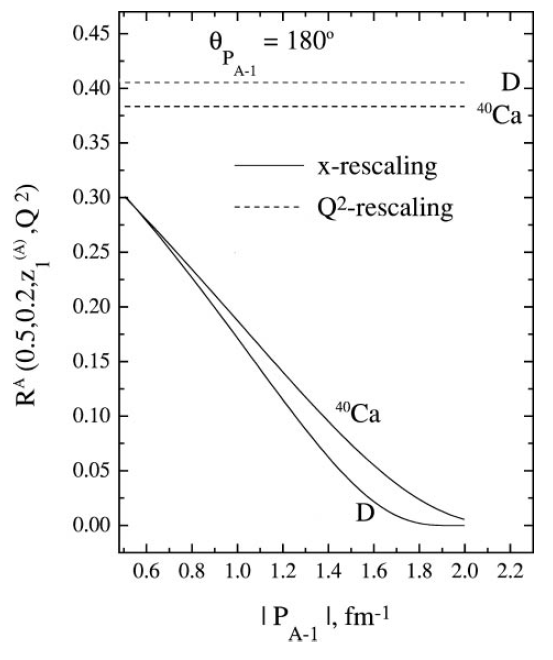
\includegraphics[angle=0, width=0.42\textwidth]{./fig-chap1/ratio_a}
    \caption{The ratio $R^A(x_B,x'_B)$ for $A = 2$ and $A = 40$, $x_B = 0.2$ and $x'_B = 0.5$, $Q^2 = 20$ GeV/$c$, plotted versus the momentum of the recoil nucleus ($A-1$) at perpendicular (left) and backward (right) angle $(\theta_{P_{A-1}} = 180^{\circ})$. The full and dashed curves are predictions of the $x$-scaling (binding) and $Q^2$-rescaling models, respectively.}
    \label{fig:ratio_a}
  \end{center}
\end{figure}

\section{Local EMC effect}

\begin{figure}
  \begin{center}
    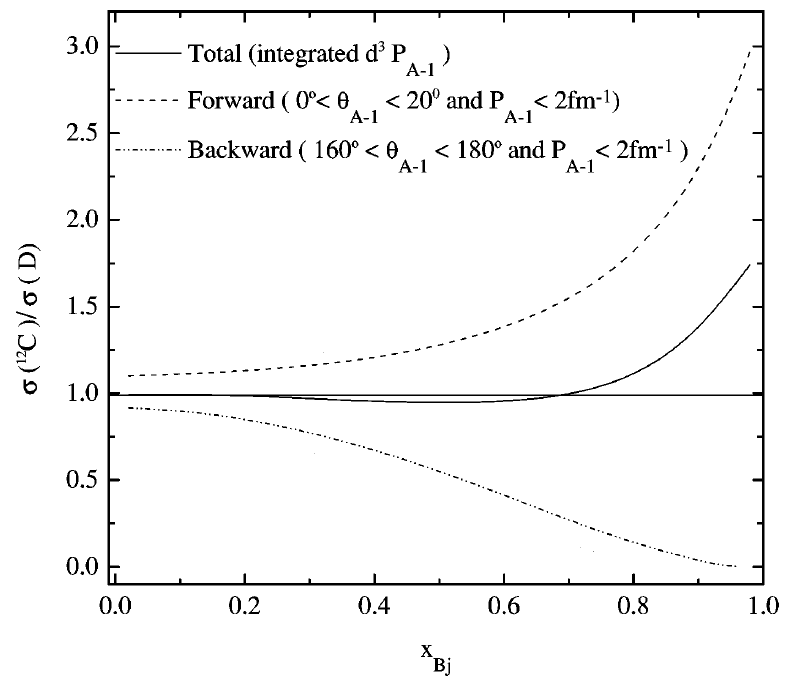
\includegraphics[angle=0, width=0.6\textwidth]{./fig-chap1/ratio_0}
    \caption{The semi-inclusive EMC ratio $R_0(x,Q^2)$ versus $x$ with nuclei emitted forward and backward, the full curve is the usual inclusive EMC ratio, the dashed and dotted curves are predictions for the local EMC effect for different spectator recoil angles~\cite{CiofidegliAtti1999} (see the legend).}
    \label{fig:r0}
  \end{center}
\end{figure}

The semi-inclusive reactions also provide a unique opportunity to investigate the local EMC effect~\cite{Kumano1990,ciofiliuti1991,CiofidegliAtti1999}. The recent data on $^9$Be indicate that the local nuclear environment may play an important role~\cite{Seely2009}. In the binding model framework~\cite{frankfurt1988}, the EMC ratio is generated by an average value of the nucleon removal energy, which depends strongly on the shell of the nucleon. Theoretical calculations show that the semi-inclusive EMC ratio,
\begin{equation}
R_0 (x,Q^2) =\frac{\int_a^b\sigma_1^Ad\vec P_{A-1}}{\int_a^b\sigma_1^Dd\vec P_{A-1}},
\label{eq:semi_emc}
\end{equation}
in which the cross section is integrated over a small momentum range of the recoil nucleus $\vec P_{A-1}$, has opposite behavior for recoil nuclei emitted forward versus backward (Fig.~\ref{fig:r0}). This leads to deviations much larger than the usual inclusive EMC effect and provides opportunity for a significant experimental check of the binding models.

\section{Flavor dependent parton distribution functions}

Measurements of tagged structure functions have been carried in CLAS by the e6 run group to study the EMC effect in deuteron \cite{klimenko2006} and later by the BoNuS collaboration \cite{bonus6} to extract the $F^n_2$ structure function by tagging the low momentum recoil proton. The main goal of the BoNuS measurements is to extract the ratio $F^n_2/F^p_2$ at high $x$ and therefore access the ratio of down to up quark distribution ($d/u$) \cite{Baillie:2011za}. By using $^4$He targets and tagging the recoiling $^3$He and $^3$H nuclei, one can select scattering off a weakly or deeply bound neutron and proton respectively depending on their off-shellness in the $^4$He nucleus. Since bound neutrons are always off-shell, even when $P_{^3He}=0$, an extrapolation procedure is needed to extract the free (i.e. on-shell) neutron structure function from the tagged recoil data \cite{Sargsian:2005rm}. One could measure the $F_2$ structure functions of a weakly bound neutron in $^4$He and compare it to the $^2$H data to detect any nuclear dependence. This procedure is necessary for neutrons due to the absence of a free neutron target. It can also be quantitatively benchmarked using the $^4$He tagged data for scattering off a weakly bound proton, and comparing the results to the well measured free proton structure functions.

In addition, the ratio $\left(F_2^n/F_2^p \right)^{bound}/ \left(F_2^n/F_2^p \right)^{free}$ can be measured to extract the distributions of $d/u$ in a free nucleon and compare it to the same ratio for bound nucleon. This is one of the way to explore the flavor dependent nuclear parton distributions which are little known experimentally. Such an effect, either in the antishadowing or EMC region, has been widely used to explain the NuTeV anomaly~\cite{Brodsky:2004qa,Cloet2009}. %There is probably other refs.


